\chapter{Análisis}\label{chap:Analisis}
En el capítulo anterior se listaron distintas tecnologías que podían sernos útiles para nuestro proyecto. En el actual nos detendremos a explicar cuáles de ellas explicaremos y el por qué de su elección.

\section{Simulador de redes: GNS3}
Se ha decidido que GNS3 sea el simulador de redes a utilizar para nuestro proyecto por varias razones:
\begin{itemize}
\item Es \textbf{multiplataforma}, con lo que podemos trabajar sencillamente con él tanto desde Windows como Linux.
\item Existe \textbf{mucha información} para consultar. Desde internet contamos con documentación oficial y un foro propio. Hay incluso libros sobre él y como ejemplo tenemos el usado en varias ocasiones en este documento, ``The Book of GNS3'', por Jason C. Neumann.
\item Es altamente \textbf{expandible}: hay decenas de aparatos reales que pueden incluirse y emularse en las topologías creadas. Pueden descargarse desde \MYhref{https://www.gns3.com/marketplace/appliances}{su marketplace}.
\item \textbf{Cuenta con una API REST} que lo hace interactivo desde el exterior.
\item Integra \textbf{WireShark} nativamente para estudiar el envío de datos entre los distintos dispositivos.
\end{itemize}

GNS3 se estructura en \textbf{proyectos}. En cada proyecto podemos desplegar una serie de dispositivos y conectarlos entre sí. Al guardar un proyecto como tal, el despliegue realizado se guarda junto a él. Sin embargo, el estado de las máquinas no corre la misma suerte, y es que a cada apagado de las mismas toda su configuración se pierde.

Una de las características más interesantes de GNS3 y sus proyectos está en la importación y exportación de estos. El simulador cuenta con una opción que permite extraer todo un proyecto en una imagen (de formato \textit{.gns3project}) para que sea fácilmente portable. Existe la posibilidad de exportar, junto a la topología creada, las imágenes base sobre las que los nodos del proyecto están construidas para que no sea necesario contar con esas imágenes en el GNS3 donde se pretende importar.

\begin{figure}[h]
  \centering
  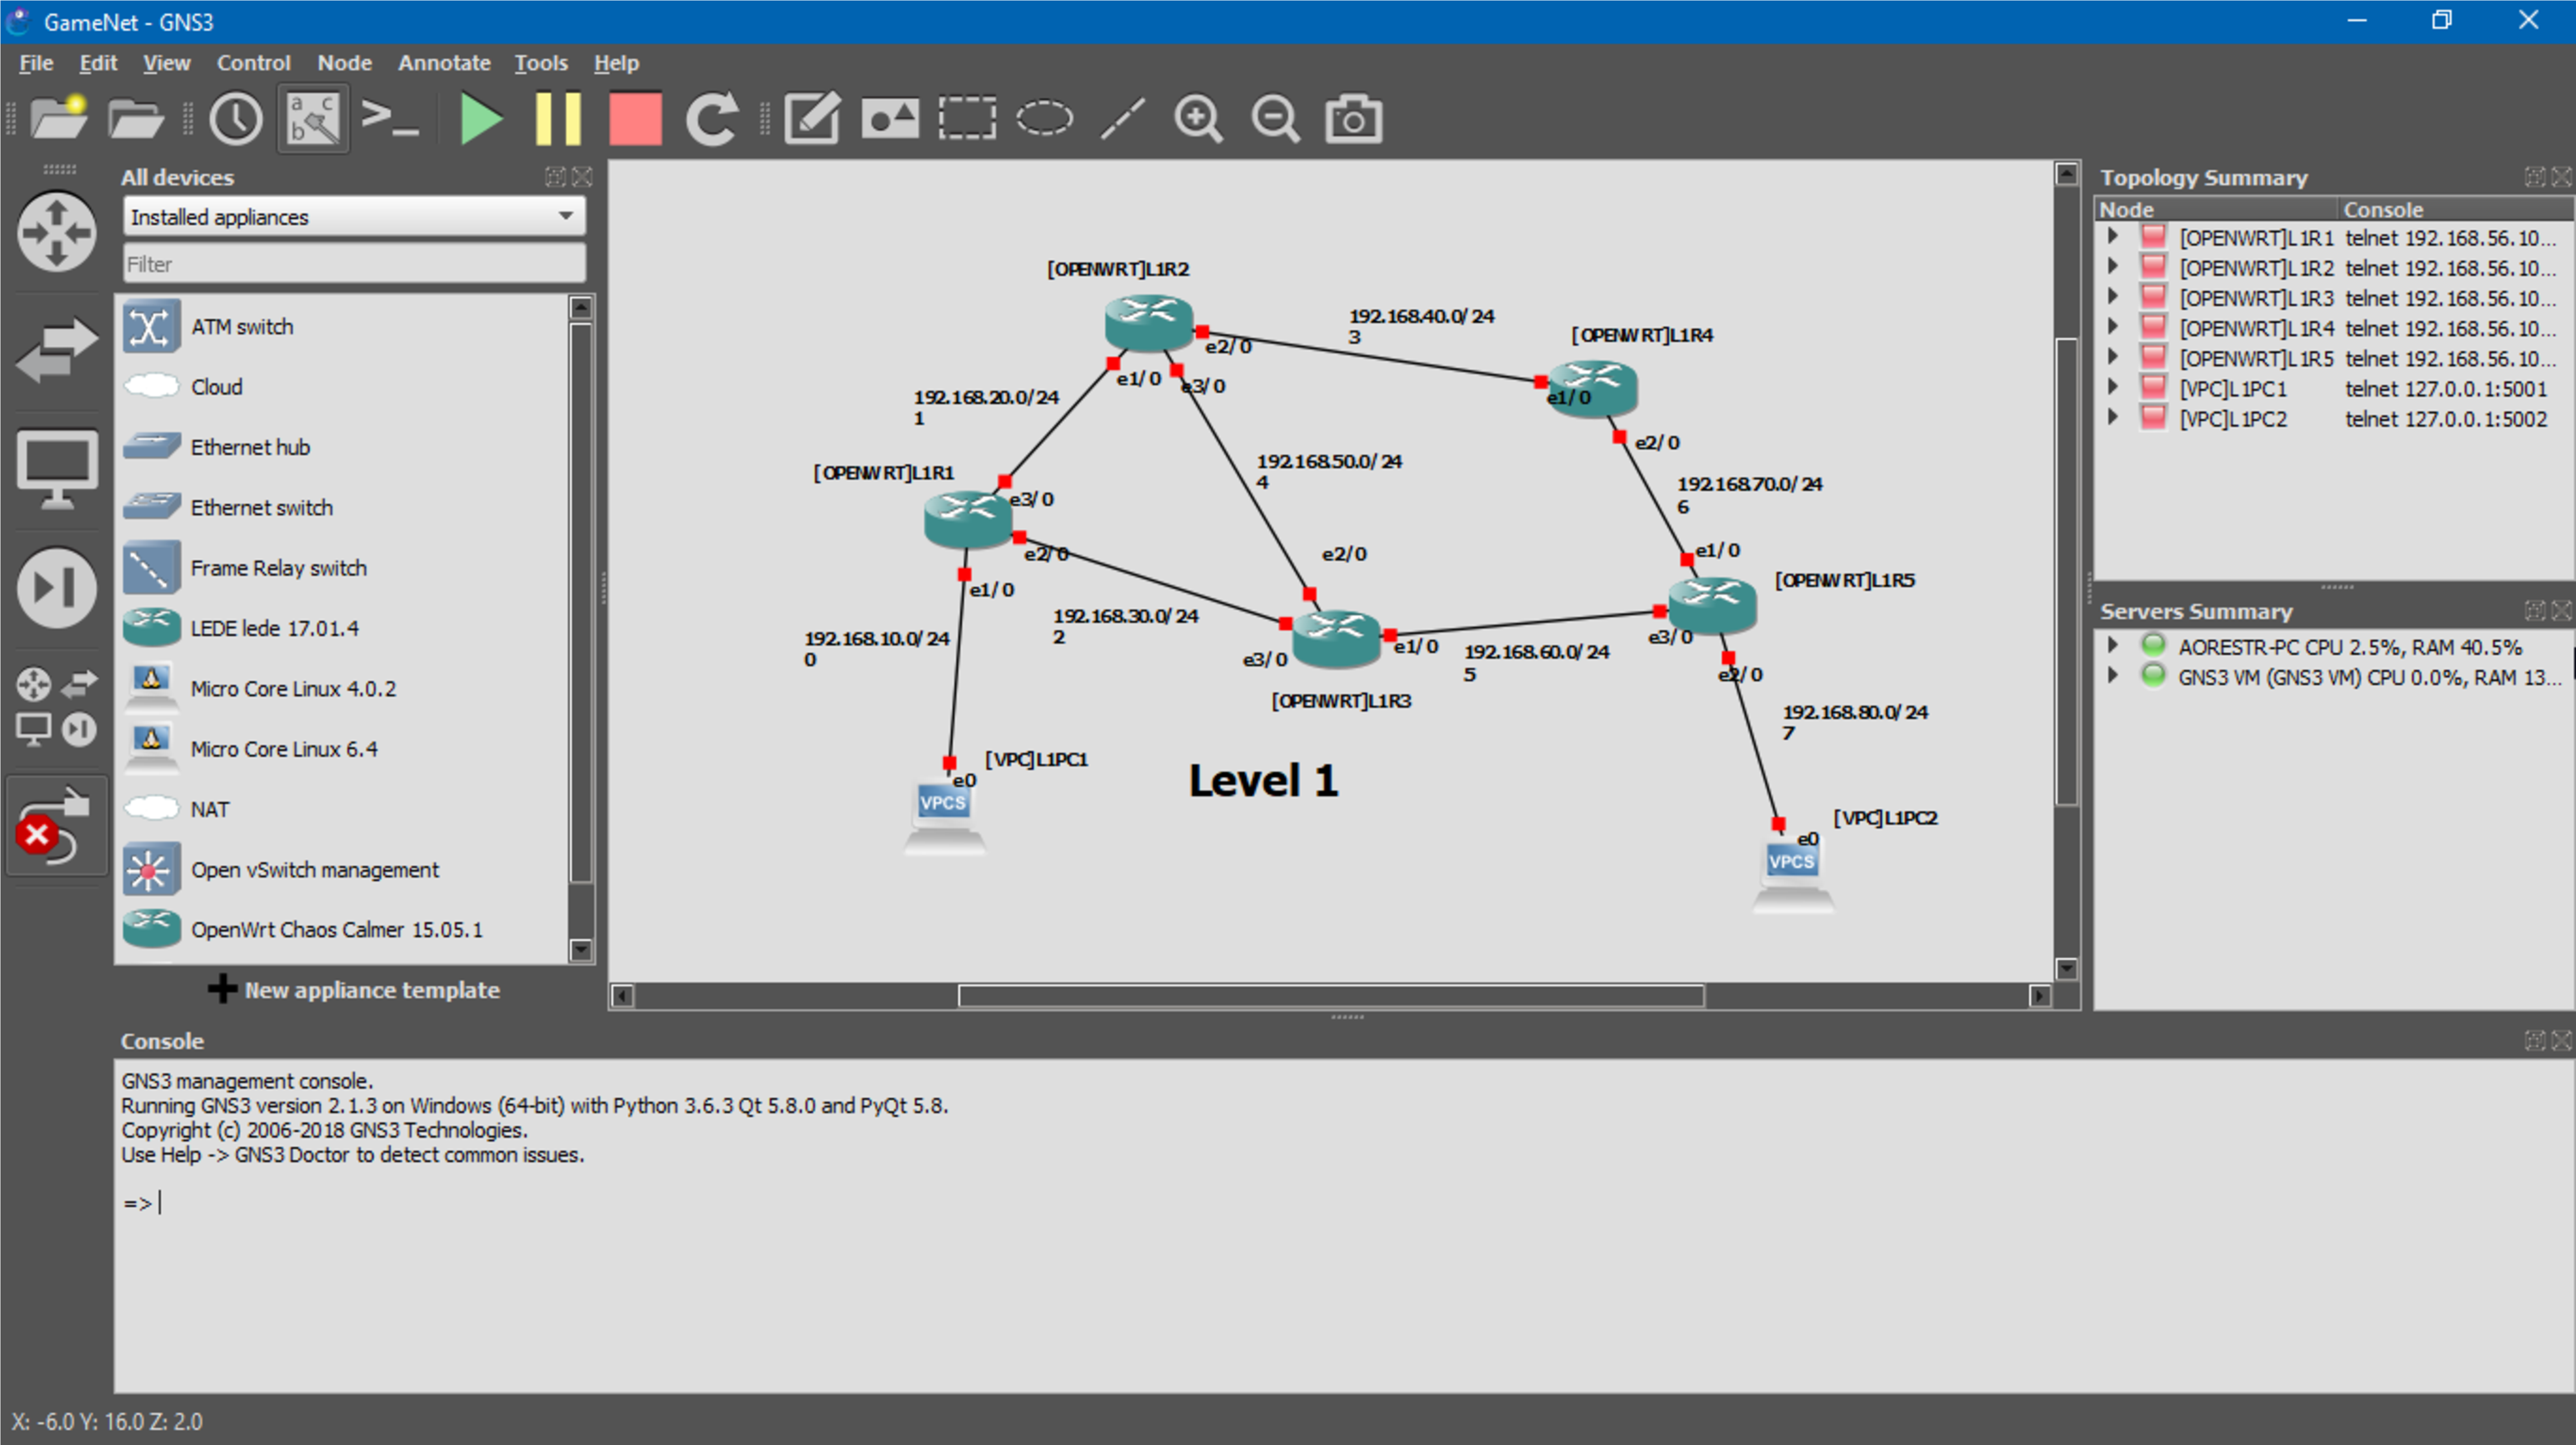
\includegraphics[scale=0.15]{imagenes/interfazgns}
  \caption{Interfaz de GNS3}
  \label{fig:interfazgns}
\end{figure}

La interfaz de usuario de la aplicación puede verse en la figura \ref{fig:interfazgns}. La barra de arriba está repleta de opciones relacionadas con el proyecto, como arrancar todos los dispositivos, pausarlos, pararlos o incluso herramientas de dibujo para convertir el esquema en algo más intuitivo y legible. A la izquierda se listan los nodos disponibles en la máquina. Arrastrándolos al centro los insertamos en el proyecto.

A continuación pasaremos a explicar conceptos clave del emulador.

\subsection{Arquitectura de GNS3}
La documentación de GNS3 recoge el modo en el que la aplicación está estructurada. La ilustración \ref{fig:estructuragns3} está sacada directamente de ella \cite{structuregns3}.

\begin{figure}[h]
  \centering
  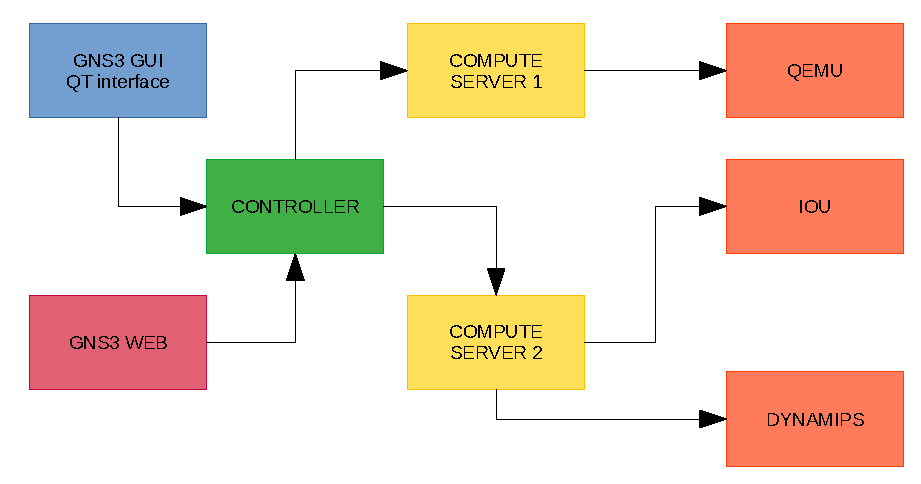
\includegraphics[scale=0.6]{imagenes/estructuragns3}
  \caption{Estructura interna de GNS3}
  \label{fig:estructuragns3}
\end{figure}

Las distintas partes que componen la aplicación se transmiten la información sobre HTTP haciendo uso de mensajes JSON (del inglés, \textit{JavaScript Object Notation}), un formato de intercambio de datos ligero fácil de leer y escribir para humanos \cite{JSON}.

Volviendo a la imagen, el controlador (\textit{controller}) controla todo la parte que gestiona el estado de un proyecto y lo guarda en el disco. Sólo existe un controlador para toda la aplicación. El GUI o interfaz de usuario es la encargada de mostrar las topologías. Toda la información que necesita la toma directamente del controlador. En los ``compute'' es donde se ejecutan los emuladores. Para cada aparato de la topología se inicia una instancia de emulador.

\subsection{El servidor}
El controlador y los ``compute'' de GNS3 forman el servidor del mismo. GNS3 aprovecha la tecnología cliente-servidor; al igual que un navegador web se conecta a un servidor web para acceder a las páginas web y mostrarlas, el GUI accede al servidor, permitiendo que se inicie, pare y controlar los dispositivos desplegados. Esto permite que los proyectos sean fácilmente escalables, ya que no necesitan ser ejecutados en un único equipo. Si se pretende trabajar con topologías grandes o complejas, también se puede ejecutar el servidor GNS3 en un PC diferente a aquel donde el GUI es ejecutado. Por consiguiente, de contar con un servidor de altas prestaciones, es posible instalar el servidor de GNS3 allí y desde otro sistema remoto construir y controlar las redes \cite{bookgns}.

\subsection{La API}
GNS3 habilita la interacción con el servidor mediante una API REST (cuyo significado será explicado en la sección \ref{subsec:sectionapi}). Mediante el protocolo de red HTTP es posible construir proyectos y llenarlos con nodos y enlaces (que se definirán a continuación) sin necesidad de hacer uso de la interfaz de usuario. En la breve \MYhref{https://gns3-server.readthedocs.io/en/latest/curl.html}{documentación de la API} oficial es posible ver algunos ejemplos de uso.

GNS3 se encarga de asignar a cada proyecto un ID único. Un ejemplo de recurso puede ser el siguiente, donde se accede a un JSON con los proyectos abiertos en GNS3 e información básica sobre ellos: \textit{http://$<$IP del server$>$:$<$puerto del servidor$>$/v2/projects}.

\subsection{Nodos}
Cada dispositivo de una red está representado en GNS3 por un elemento llamado \textbf{nodo}. Estos nodos, que pueden ser desde un router a un switch, no son más que virtualizaciones de aparatos reales. Por norma general, las virtualizaciones se realizan a partir de imágenes de los sistemas operativos que se integran en los aparatos. Así, podemos tener varios routers distintos de Cisco montados sobre la misma estructura, permitiéndonos jugar con ellos con verdadera facilidad.

Tanto en macOS como en Windows es necesario utilizar \textbf{GNS3 VM} para hacer uso de ciertos nodos. Se trata de una imagen con un Ubuntu ligero que se instala en un hipervisor (VMware, Virtualbox) y hace de sistema operativo desde el que ejecutar los aparatos que se implanten en la red. Las ventajas de usar GNS3 VM son las siguientes \cite{gns3vm}:
\begin{itemize}
\item Algunas dependencias son difíciles de instalar, como los requisitos para IOU; necesitan una librería específica.
\item Con VMware es posible utilizar utilizar la aceleración KVM para QEMU.
\item Dynamips y QEMU funcionan mejor en Linux (menos problemas aleatorios con ASA por ejemplo).
\item Soporte completo de IOU.
\item No hay antivirus o firewall dentro de la máquina virtual que modifique el tráfico de la red.
\item La máquina está aislada del host, lo que implica un mayor nivel de seguridad.
\end{itemize}

Los nodos pueden ser inicializados juntos (todos los del proyecto a la vez) o por separado. GNS3 los asigna a un puerto de la red desde el que pueden ser accedidos y controlados mediante telnet.

En la API, para obtener los distintos nodos que existen un proyecto es necesario acceder al recurso: \textit{http://$<$IP del server$>$:$<$puerto del servidor$>$/v2/projects/$<$ID del proyecto$>$/nodes}

\subsection{Enlaces}
Los nodos están interconectados entre sí mediante enlaces. Los enlaces son los encargados del envío de paquetes entre ellos. Sus características pueden ser modificados mediante ``filtros de paquete'' (\textit{Packet filters}), que no son más que unos parámetros que afectan a las conexiones. Desde la latencia a la probabilidad de pérdida de paquetes se puede controlar mediante ellos.

El recurso asociado en la API a los enlaces de un proyecto es: \textit{http://$<$IP del server$>$:$<$puerto del servidor$>$/v2/projects/$<$ID del proyecto$>$/links}
 
\section{Motor de videojuegos: Unity}
realmente esta elección no era tan complicada